\chapter{Method}

The method chapter of this paper describes the process of generating Neural Radiance Fields (NeRFs). We will cover the five key steps involved in the NeRF generation process: capture, process, training, rendering, and evaluating. Lastly we'll have a look at the dataset captured and used throughout the experiments.

Our approach to generating NeRFs leverages state-of-the-art software that allows us to test and compare multiple different methods. We have selected a range of methods to evaluate, including traditional and cutting-edge techniques. This will provide valuable insights into the strengths and limitations of different approaches to NeRF generation.

In the capture step, we will describe the process of acquiring the necessary data to train the NeRF model. This includes details of the equipment and techniques used to capture high-quality images of real-world scenes. The process step involves preprocessing the captured data to prepare it for use in training the NeRF model. This includes tasks such as downscaling, feature extraction, and global adjustment of the input data. We will describe the specific methods and algorithms used for these tasks. The training step is where the NeRF model is actually learned from the processed data. In the rendering step, we will describe how the trained NeRF model is used to generate novel images of the scene. Finally, in the evaluating step, we will describe how we quantitatively and qualitatively assessed the quality of the generated NeRFs. Overall, this method chapter provides a description of the process of generating NeRFs, from data capture to evaluation.

%We will describe the specific neural network architecture and training algorithms used, as well as the hyperparameters that were applied. %We will also discuss any challenges or obstacles that we encountered during training, and how we addressed them. 

\begin{comment}
Describe the pipeline used to generate NeRFs

- Capture (video, image, polycam, etc.)
- Process (COLMAP, or direct extraction from e.g. Polycam)
    - Configuration of COLMAP
- Train (Different models)
    - Configuration of model
- Render (Real-time rendering vs. slow rendering)
- Evaluate (PSNR, SSIM, LPIPS)
- Export

- Pipelines created
    - Pipeline to test 
\end{comment}

\section{Nerfstudio}
With the magnitude of different published methods regarding NeRF, some with corresponding source code and some not, it's not trivial to compare them on self-captured data. In the experiments, I have leveraged an open-source project named Nerfstudio \cite{nerfstudio}. It is an API that streamlines the creation, training, and visualization of NeRFs. The components that make up NeRFs are modularized in a way that allows interpretable implementation of different NeRF methods. In addition, it ships with implemented versions of some of the most important published methods to date for real-world captures; NeRF, mip-NeRF, and instant-ngp.

\section{Nerfacto}
Nerfstudio also provides its own method dubbed "Nerfacto". The method isn't published work, but leverages techniques from several other published methods which have proved to work well for real data captures. The techniques used in Nerfacto result in a method that strikes a great balance between quality and speed. The techniques highlighted by Nerfacto have already been discussed in \autoref{chap:relatedwork}, but I'll recap and elaborate on a few here.

\begin{figure}[!h]
    \centering
    %\hspace*{-48px}
    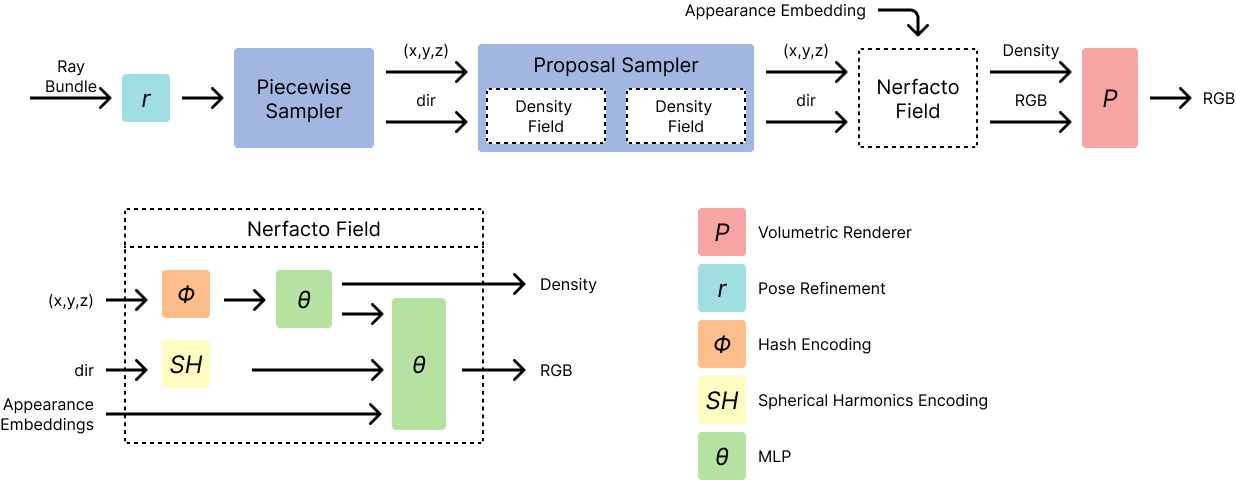
\includegraphics[width=1.0\textwidth]{figures/nerfacto-pipeline-overview.png}
    \caption{}
    \label{fig:nerfacto-pipeline-overview}
\end{figure}

\textbf{Camera pose refinement}, as described in \autoref{sec:camera-pose-refinement} is a technique proposed to reduce the impact of imperfect camera poses. It's a very effective measure to reduce cloudy artifacts and increase the sharpness and overall quality of the resulting 3D representation.

\textbf{Per image appearance conditioning}, as described in \autoref{sec:appearance-embeddings}, is a technique that allows the NeRF to process and represent 3D scenes with variable lighting, exposures, weather, and post-processing effects. In Nerfacto, the appearance embedding is a vector of size 32, which is concatenated with the viewing direction before it's passed through the MLP.

\textbf{Hash encodings}, as described in \autoref{sec:instant-ngp}, is an effective encoding scheme used to severely decrease training- and inference time. In Nerfacto, 16 hash tables with $2^{19}$ rows, each storing a feature vector of size 2, are allocated. The subsequent MLP has a very low capacity, with only one hidden layer containing 64 neurons.

\textbf{Proposal sampling}, as described in \autoref{sec:mipnerf360}, is a sampling technique used to increase the sampling density of areas that contribute most to the final render. Nerfacto extends the proposal sampler used in mip-NeRF 360 \cite{barron_mip-nerf_2022} by utilizing two density functions implemented as small fused-MLP with hash encodings \cite{muller_instant_2022}. This provides accurate and fast density estimations.

\textbf{Scene contraction}, as described in \autoref{sec:mipnerf360}, is a technique proposed in mip-NeRF 360 \cite{barron_mip-nerf_2022} to extend mip-NeRF to support unbounded scenes.

\section{Capture}
The different datasets have primarily been captured with an iPhone 13 Pro Max. The iPhone features three lenses that enable captures ranging from ultra-wide to telephoto. Using the ultra-wide option has proved helpful in the pipelines where COLMAP has to be leveraged, as it captures more of the scene and more easily enables overlap between the frames. The resulting NeRF-renderings haven't seemed distorted. When capturing video or images for a NeRF it's important that the scene is well-lit, that you capture non-blurry images, and that there are no transient objects present.

Polycam is a "LiDAR \& 3D Scanner for iPhone \& Android". It has multiple settings for performing photogrammetry and LiDAR scans, but most importantly it enables export of images with corresponding camera poses. This is very useful as Nerfstudio has created an integration that reads the camera poses generated by Polycam and transforms it into Nerfstudio's data format. This enables skipping COLMAP entirely from the pipeline. Polycam doesn't support wide camera options, resulting in the need to manually record more of the scene.
%The quality of the camera poses are relatively good.

Both regular capture through the iPhone's own camera-app, and through Polycam have been conducted in order to gather data for the succeeding experiments.

\section{Process}
The data processing step for constructing a NeRF are usually the same across different models. It's a step for creating the dataset of images with corresponding camera poses and is comprised of creating a set of images from a video, scaling the images to a preferred size, and lastly utilizing an algorithm to extract the corresponding camera poses. If you a priori have access to the input images and refined camera poses, as is the case when utilizing the Polycam, there's not much pre-processing necessary. All the experiments in this paper leverage Nerfstudio which has its own data processing pipeline API that includes support for video, images, and Polycam-data. For video input, FFMPEG \cite{tomar2006converting} is first used to grab image frames from the video at specified densities, by default $\sim$300 frames. When a set of images is acquired, the images are scaled down in fractions of the original image size. The scaling of the images is done as it's been obeserved that training on images larger than 1600px along the longest dimension has diminishing returns. COLMAP is then used for extracting the camera poses from the set of input images. The choice of matching algorithm, as discussed in \autoref{sec:sfm}, is primarily the only setting you have to tweak for COLMAP.

\begin{lstlisting}[
    caption={Example of running Nerfstudio's process-script. Reference the \href{https://docs.nerf.studio/en/latest/index.html}{documentation} for details.},
    label=code:process,
    language=bash]
$ data_path={nerfstudio/data/your-data-folder}
$ ns-process-data {video, images, polycam} --data $data_path 
  --output-dir $data_path/output
\end{lstlisting}

%COLMAP and FFMPEG \cite{tomar2006converting} are the main data processing tools. FFMPEG is used to grab image frames from the video at specified densities, by default ~300 frames. COLMAP is then used for extracting the camera poses from a set of input images. The choice of matching algorithm, as discussed in \autoref{sec:sfm}, is primarily the only setting you have to tweak for COLMAP.
%Most of the experiments use the default number of frames and the default COLMAP matching algorithm.

\section{Train}
%- Configuration of model
During training, the parameters in the model are trained to represent the 3D scene. For the Nerfacto-model, this entails backpropagating the error and updating both the NeRF MLP and the proposal MLP. For the instant-ngp-model, the small MLP and the feature vectors contained in the multiresolution hash tables are updated.

The training has been conducted with different models, varying amounts of data, and for different scenes. All the configurations have been adjusted with Nerfstudio's API. By default, the dataset is created from $\sim$300 frames and the corresponding camera poses. The "fast" methods, instant-ngp and Nerfacto, have been trained for 30'000 steps. The "slow" methods have been trained for 32 hours, resulting in $\sim$500'000 steps. The specific parameters for each model are shown in \autoref{app:additional}.

\begin{lstlisting}[
    caption={Example of running Nerfstudio's train-script with the nerfacto model. Reference the \href{https://docs.nerf.studio/en/latest/index.html}{documentation} for details.},
    label=code:train,
    language=bash]
$ data_path={nerfstudio/data/your-data-folder}
$ ns-train nerfacto --data $data_path
\end{lstlisting}

\section{Render}
%- Real-time rendering vs. slow rendering
During rendering, the trained NeRF is queried along a camera path to output a series of images. The camera path contains information about the keyframes to be rendered, the camera-to-world matrices, and data such as render height and width, FPS, and video duration. In Nerfstudio, a camera path can simply be created in their real-time rendered viewer. The camera path can later be exported and used across models trained on the same data to qualitatively compare them.

%The render output can also be tweaked by tuning sampling rates contained in the \textit{config.yml}-file that is generated after you've trained the NeRF.

\begin{lstlisting}[
    caption={Example of running Nerfstudio's render-script. Reference the \href{https://docs.nerf.studio/en/latest/index.html}{documentation} for details.},
    label=code:render,
    language=bash]
$ data_path={nerfstudio/data/your-data-folder}
$ output_path={nerfstudio/outputs/.../nerfstudio_models}

$ ns-render --load-config $data_path/config.yml --traj filename 
  --camera-path-filename $output_path/camera_path.json
\end{lstlisting}




\section{Evaluate}
%Evaluation scripts
In order to evaluate the NeRF we can use the metrics discussed in \autoref{sec:evaluating-nerfs}. Nerfstudio provides a script for loading a checkpoint and computing the related PSNR, SSIM, and LPIPS. These metrics give a great quantitative impression of the quality of the resulting NeRF, but there is a lot of value in the qualitative output as well. All the trained NeRFs in this paper are also rendered in order to visually compare the results across methods, configuration and data.

\begin{lstlisting}[
    caption={Example of running Nerfstudio's built-in evaluation script. Reference the \href{https://docs.nerf.studio/en/latest/index.html}{documentation} for details.},
    label=code:eval]
$ config_path={nerfstudio/outputs/.../nerfstudio_models/config.yml}
$ ns-eval --load-config $config_path
\end{lstlisting}


\section{Pipelines for testing}
%Discuss the different pipelines I've created to test different methods against each other.
In order to test multiple different methods with different parameters, data sizes, etc. I created a wrapper script around the Nerfstudio CLI. The wrapper script will process, train and evaluate a NeRF. In addition to this, it wraps each step with a timer context manager which will write time information about the different steps to a log-file.


%In Nerfstudio the processing is handled by two modular classes, namely the \textit{DataParser} and \textit{DataManager}. The \textit{DataParser} is responsible for parsing the input-data, e.g. the raw Polycam-data, into a standard data format. The data format contains information about the camera intrinsic and extrinsics. The intrinsics contain information about the camera used for capture, e.g. the focal length, image dimensions and possible radial distorial parameters. The extrinsics couples an input-image to a transform matrix. After the data has been parsed, it is passed to the the \textit{DataManager} that is responsible for supplying bundles of rays and the corresponding ground truth information.

%In Nerfstudio during training, the \textit{DataManager} passes ray bundles and ground truth information to a model. The model samples points along the provided rays and passes it to a contained \textit{Field}. A simple field takes in a 3D location and viewing direction and outputs density and color.

\section{Dataset} \label{sec:dataset}
The dataset used throughout this report contains self-captured data alongside data from previous NeRF papers. It contains examples of synthetic scenes (Blender scenes), forward-facing scenes, unbounded scenes, and large, unbounded outdoor scenes.

\begin{figure}[!h]
    \centering
    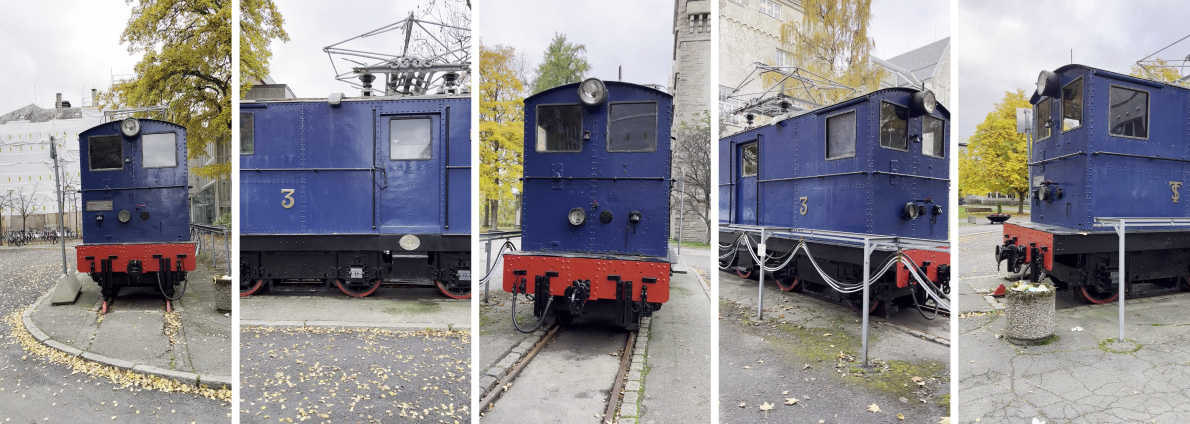
\includegraphics[width=1.0\textwidth]{figures/ohma_electra.png}
    \caption{Unbounded scene: The dataset of Ohma Electra is ~47 seconds long, captured at 30 FPS. The dataset contains 1416 images.}
    \label{fig:ohma-electra}
\end{figure}
\begin{figure}[!h]
    \centering
    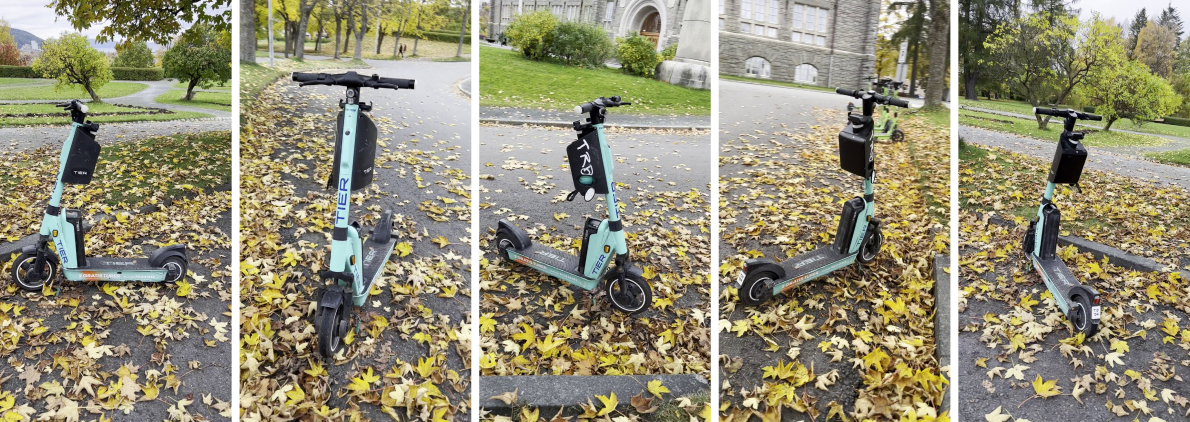
\includegraphics[width=1.0\textwidth]{figures/tier.png}
    \caption{Unbounded scene: The dataset of an electric scooter is ~15 seconds long, captured at 30 FPS. The dataset contains 446 images}
    \label{fig:tier}
\end{figure}

\begin{figure}[!ht]
    \centering
    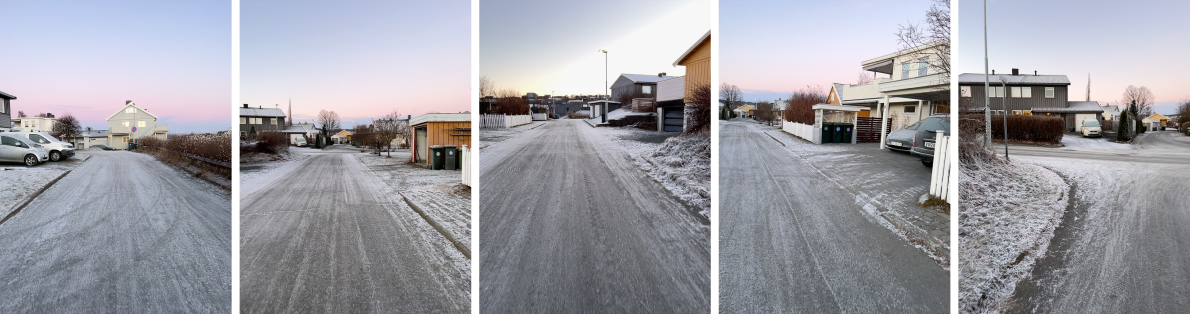
\includegraphics[width=1.0\textwidth]{figures/streetview-dataset.png}
    \caption{Large outdoor, unbounded scene: The dataset of a street in Trondheim is originally caught with the Polycam app. The dataset contains 600 images.}
    \label{fig:streetview-dataset}
\end{figure}
%\begin{figure}[h]
    \centering
    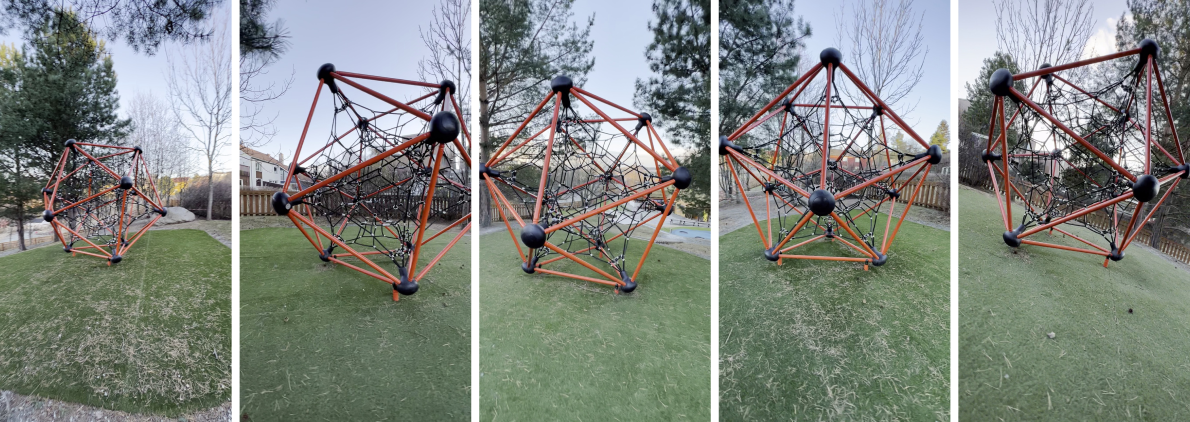
\includegraphics[width=1.0\textwidth]{figures/octahedron-dataset.png}
    \caption{Octahedron dataset. Caught with an iPhone at 0.5x zoom.}
    \label{fig:octahedron-dataset}
\end{figure}
\begin{figure}[h]
    \centering
    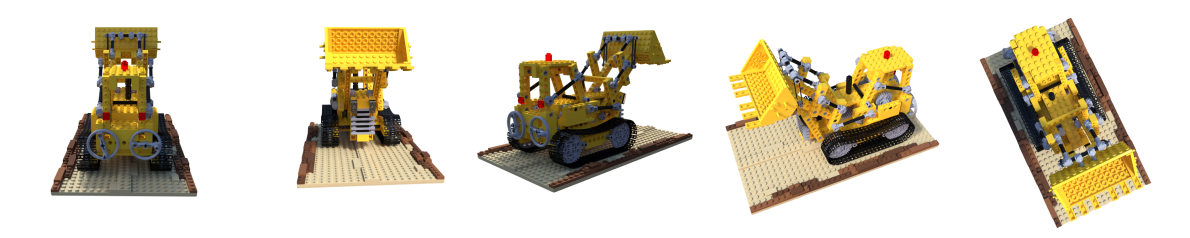
\includegraphics[width=1.0\textwidth]{figures/lego-dataset.png}
    \caption{Blender scene: The dataset of a lego tractor. This dataset is one of the benchmarks in the original NeRF paper. The dataset contains 100 images.}
    \label{fig:lego-dataset}
\end{figure}
\begin{figure}[!h]
    \centering
    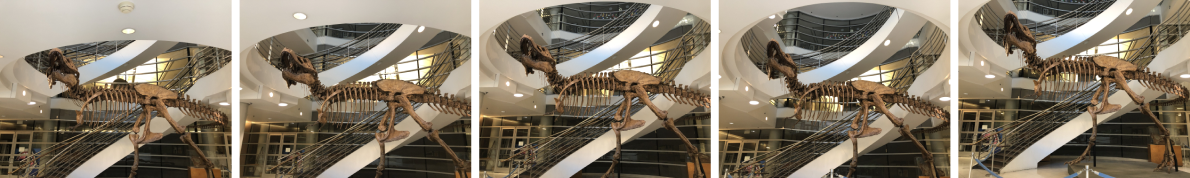
\includegraphics[width=1.0\textwidth]{figures/trex-dataset.png}
    \caption{Forward-facing scene: Contrary to the other scenes, this scene's images are all captured in a 2D plane along the X- and Y-axis, assuming Z is the axis parallel to the viewing direction. The dataset is from the original NeRF paper \cite{mildenhall_nerf_2020}. The dataset contains 56 images.}
    \label{fig:trex-dataset}
\end{figure}

\begin{figure}[h]
    \label{fig:fox-dataset}
    \centering
    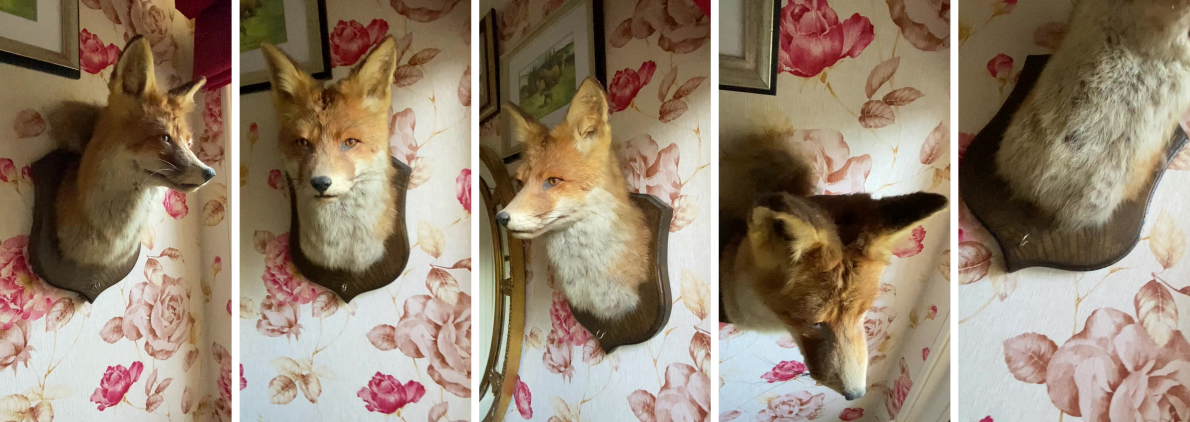
\includegraphics[width=1.0\textwidth]{figures/fox-dataset.png}
    \caption{Bounded scene: The dataset of a stuffed fox on a wall. This dataset is one of the datasets from the instant-ngp repository.}
    \label{fig:my_label}
\end{figure}